\documentclass[border=5mm]{standalone}
\usepackage{tikz}
\usepackage{pgfplots}
\usetikzlibrary{patterns}
\pgfplotsset{compat=1.10}
\usepgfplotslibrary{fillbetween}
\usetikzlibrary{intersections}
\begin{document}
  方法一:
  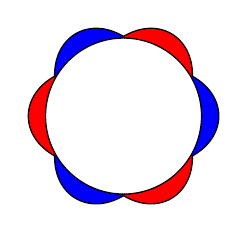
\begin{tikzpicture}[scale=1]
    \def\R{1}
    \def\s{0.2}

    \foreach \d in {-pi/6:pi/6,pi/2:5/6*pi,-pi/2:-5*pi/6
    }{
    \draw [black, line width=1pt,samples=100,domain=\d, name path=B]
    plot ({(\R + abs(\s*cos(3*\x r)))*cos(\x r)}, {(\R + abs(\s*cos(3*\x r)))*sin(\x r)});
    \draw [black, line width=1pt,samples=100,domain=\d, name path=A]
    plot ({\R*cos(\x r)}, {\R*sin(\x r)});
    \tikzfillbetween[of=B and A]{blue};
    }

    \foreach \d [count=\c] in {pi/2:pi/6,5*pi/6:7*pi/6,3*pi/2:11*pi/6
    }{
    \draw [black, line width=1pt,samples=100,domain=\d, name path=C]
    plot ({(\R + abs(\s*cos(3*\x r)))*cos(\x r)}, {(\R + abs(\s*cos(3*\x r)))*sin(\x r)});
    \draw [black, line width=1pt,samples=100,domain=\d, name path=A]
    plot ({\R*cos(\x r)}, {\R*sin(\x r)});
    \tikzfillbetween[of=A and C]{red};
    }
  \end{tikzpicture}

  \par 方法二:
  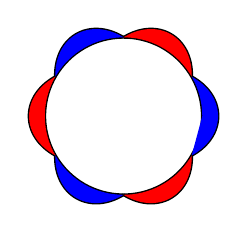
\begin{tikzpicture}[scale=1]
    \def\R{1}
    \def\s{0.2}

    \draw [black, line width=1pt,samples=100,domain=0:2*pi, name path=A]
    plot ({\R*cos(\x r)}, {\R*sin(\x r)});

    \draw [black, line width=1pt,samples=100,domain=-pi/6:pi/6, name path=B]
    plot ({(\R + abs(\s*cos(3*\x r)))*cos(\x r)}, {(\R + abs(\s*cos(3*\x r)))*sin(\x r)});

    \draw [black, line width=1pt,samples=100,domain=pi/6:pi/2, name path=C]
    plot ({(\R + abs(\s*cos(3*\x r)))*cos(\x r)}, {(\R + abs(\s*cos(3*\x r)))*sin(\x r)});

    \draw [black, line width=1pt,samples=100,domain=pi/2:5/6*pi, name path=D]
    plot ({(\R + abs(\s*cos(3*\x r)))*cos(\x r)}, {(\R + abs(\s*cos(3*\x r)))*sin(\x r)});

    \draw [black, line width=1pt,samples=100,domain=5*pi/6:7*pi/6, name path=E]
    plot ({(\R + abs(\s*cos(3*\x r)))*cos(\x r)}, {(\R + abs(\s*cos(3*\x r)))*sin(\x r)});

    \draw [black, line width=1pt,samples=100,domain=7*pi/6:3*pi/2, name path=F]
    plot ({(\R + abs(\s*cos(3*\x r)))*cos(\x r)}, {(\R + abs(\s*cos(3*\x r)))*sin(\x r)});

    \draw [black, line width=1pt,samples=100,domain=3*pi/2:11*pi/6, name path=G]
    plot ({(\R + abs(\s*cos(3*\x r)))*cos(\x r)}, {(\R + abs(\s*cos(3*\x r)))*sin(\x r)});

    \fill [blue,intersection segments={of=A and B,
                    sequence={A0 -- B1[reverse]}}];
    \fill [red,intersection segments={of=A and C,
                    sequence={A1 -- B1[reverse]}}];
    \fill [blue,intersection segments={of=A and D,
                    sequence={A1 -- B1[reverse]}}];
    \fill [red,intersection segments={of=A and E,
                    sequence={A1 -- B1[reverse]}}];
    \fill [blue,intersection segments={of=A and F,
                    sequence={A1 -- B1[reverse]}}];
    \fill [red,intersection segments={of=A and G,
                    sequence={A1 -- B1[reverse]}}];
  \end{tikzpicture}

  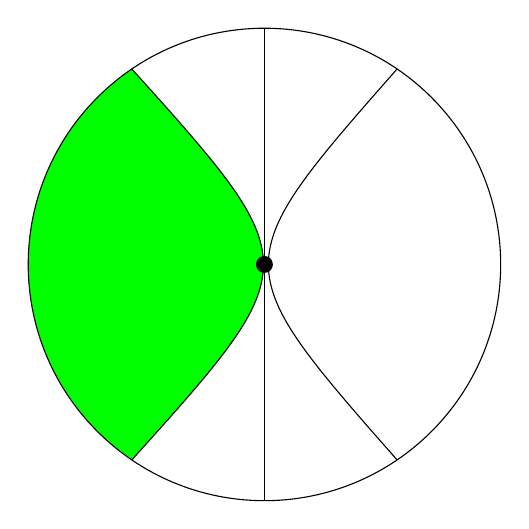
\begin{tikzpicture}
    \begin{scope}
      \clip (2,2) circle (3cm);
      \draw[fill=green]
        (current bounding box.south west) --
        (0.3,-0.5)..controls(2.55,2)..(0.3,4.5)
        -- (current bounding box.north west) -- cycle;
      \draw[] (3.7,-0.5)..controls(1.5,2)..(3.7,4.5);
      \draw (2,5)--(2,-1);
      \draw[fill] (2,2) circle [radius=0.1];
    \end{scope}
    \draw (2,2) circle (3cm);
  \end{tikzpicture}

  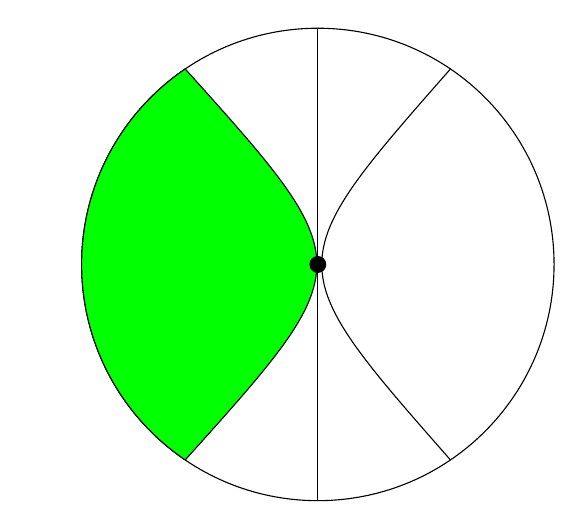
\begin{tikzpicture}
    \draw[name path = A] (2,2) circle (3cm);
    \path[name path = B] (0.3,-0.5)..controls(2.55,2)..(0.3,4.5);
    \path[name path = C] (3.7,-0.5)..controls(1.5,2)..(3.7,4.5);

    \draw (2,5)--(2,-1);
    \path[name intersections={of=A and B,by={a,b}}];
    \path[name intersections={of=A and C,by={c,d}}];
    \begin{scope}
    \clip (a) rectangle ([xshift=-2cm]b);
    \filldraw[fill=green]
      (2,2) circle (3cm);
    \end{scope}
    \begin{scope}
    \clip (a) rectangle ([xshift=2cm]b);
    \filldraw[fill=green]
      (0.3,-0.5)..controls(2.55,2)..(0.3,4.5);
    \end{scope}
    \begin{scope}
    \clip (c) rectangle ([xshift=-2cm]d);
    \draw
      (3.7,-0.5)..controls(1.5,2)..(3.7,4.5);
    \end{scope}
    \draw[fill] (2,2) circle [radius=0.1];
  \end{tikzpicture}


示例:
\begin{tikzpicture}[smooth]
\draw[arrows={-Stealth[length=5pt, inset=3.5pt]}] (-0.5,0) -- (3.0,0)node (xaxis) [right=-1pt] {$x$};
\draw[arrows={-Stealth[length=5pt, inset=3.5pt]}] (0,-0.5) -- (0,4.5)node (yaxis) [above=-0.6pt] {$y$};
\draw  (-0.18,-0.18) node {$o$};
\draw[color=red,domain=0:2.0,fill=green!20] plot (\x,4*\x-\x*\x);
\draw[color=red!40,domain=0:2.90] plot (\x,4*\x-\x*\x)  ;
\draw[color=blue!30,domain=0:2.3] plot (\x,\x)  ;
\draw[fill=black] (2,4) circle [radius=0.2pt] node[above=-1.8pt] {${A(2,4)}$};
\end{tikzpicture}

\begin{tikzpicture}[smooth]
  \draw[name path=F1,domain=-3.2:1] plot (\x,\x+1) node[right]{$x-y+1=0$};
  \draw[name path=F2,domain=-1:2] plot (\x,-\x+1) node[right]{$x+y-1=0$};
  \draw[name path=F3,domain=-3.2:2] plot (\x,\x/2-1/2) node[right]{$x-2y-1=0$};
  \draw[name path=F0,dashed,domain=-3.5:-2.5] plot (\x,-\x*2-8);
  \draw[name path=F02,dashed,domain=-0.5:2] plot (\x,-\x*2+2);
  \path[name intersections={of=F1 and F2,by=F12}];
  \path[name intersections={of=F2 and F3,by=F23}];
  \path[name intersections={of=F3 and F1,by=F31}];
  \filldraw[fill=gray,draw opacity=0.5] (F12)--(F23)--(F31)--cycle;
  \draw[arrows={->Stealth[length=5pt, inset=3.5pt]}] (-3.5,0) -- (2,0)node[below] (xaxis){$x$};
  \draw[arrows={->Stealth[length=5pt, inset=3.5pt]}] (0,-3) -- (0,3)node[left] (yaxis){$y$};
  \draw  (-0.18,-0.18) node {$O$};
\end{tikzpicture}

% \begin{tikzpicture}
%    \draw[black,name path=C] plot(\x,\x+3) node[right]{$x-y+1=0$};
%    \draw[black,name path=B] plot(\x,-\x+1) node[right]{$x+y-1=0$};
%    \draw[black,name path=A] plot(\x,(\x-1/)/2) node[right]{$x-2y-1=0$};
%    \tikzfillbetween[of=C and B,
%     split,
%     every segment no 0/.style=
%       {pattern color=gray!50,
%        pattern=north east lines},
%        ],
%     every segment no 1/.style=
%      {pattern color=white},
%       ];
% \end{tikzpicture}
\end{document}
